% -----------------------------------------------
% Articolo CIM 2026
% "Tra la sorgente e la misura:
%  influenza della catena elettroacustica e dell'ambiente sui descrittori audio"
% Taglio osservativo: cosa restituiscono i descrittori attraverso la catena;
% l'esperimento in laboratorio (distanza, doppia ripresa) e' la prova principale.
%
% Vincoli call: paper max 8 pagine; due colonne A4; IT o EN;
% abstract EN obbligatorio per autori italiani; abstract 150-200 parole.
% Scadenza sottomissione: 21 giugno 2026, 23:55 (prorogata dal 7 giugno).
% CAMERA-READY (accettato, submission 146): anonimato rimosso, autore e
% affiliazione in chiaro, brano nominato, materiale supplementare non anonimo.
% Il sorgente sottomesso in doppio cieco resta in articolo-cim2026.tex.
% Decisione 2026-06-11: prosa in prima persona singolare (diario di bordo).
% Decisione 2026-06-21: si parla normalmente del brano in prima persona
% attraverso la macro \brano; nella camera-ready rende il nome per esteso.
% File di supporto richiesti accanto a questo .tex:
%   cim2026.sty  riferimenti.bib  figura_*.pdf
% -----------------------------------------------

\documentclass{article}
\usepackage{amsmath}
\usepackage{booktabs}
\usepackage{cim2026}
\usepackage{times}
\usepackage{ifpdf}
\usepackage[english,italian]{babel}   % testo in italiano, abstract anche EN
\usepackage{float}
% variabili definite dall'utente
\def\papertitle{Descrittori audio immersi nell'ambiente: quale mappatura ricavarne}
\def\firstauthor{Francesco Ferracuti}
% Il nome del brano nel testo passa da qui.
\newcommand{\brano}{\emph{interfantasia}}

\ifpdf
  \usepackage[pdftex]{graphicx}
  \usepackage[pdftex,
    pdftitle={\papertitle},
    pdfauthor={\firstauthor},
    bookmarksnumbered,
    pdfstartview=XYZ
   ]{hyperref}
\else
  \usepackage[dvips]{epsfig,graphicx}
  \usepackage[dvips,
    bookmarksnumbered,
    pdfstartview=XYZ
  ]{hyperref}
\fi

\hypersetup{
    colorlinks,%
    citecolor=black,%
    filecolor=black,%
    linkcolor=black,%
    urlcolor=black
}

% Didascalie al corpo di default del template CIM (niente override).

\title{\papertitle}

% un solo autore: \oneauthor ; due: \twoauthors ; tre: \threeauthors
\oneauthor
  {\firstauthor} {{LEAP -- Laboratorio ElettroAcustico Permanente} \\ {\tt \href{mailto:ferracutifrancesco.00@gmail.com}{ferracutifrancesco.00@gmail.com}}}

% ***************************************** inizio documento ***********
\begin{document}
%
\maketitle

\selectlanguage{english}
\abstract
The live electronics of \brano, an ecosystemic feedback system immersed in its environment, drives its filter parameters from descriptors of the captured sound. Its original mapping drove five descriptors by their absolute values, which move with the room, not the gesture. My question: how to use a closed set of sixteen descriptors live, when the signal arrives through an environment and a chain. I gather evidence over three tests, each closer to the live signal. On synthetic signals descriptors are scale invariant yet drift under recording; on acoustic instruments the descriptor that follows the gesture depends on the instrument; and in an electroacoustic laboratory, with eight microphones over eight metres, the chain authors the measurement (air absorption, a standing wave, directivity). The three tests are the demonstrated part of this work; what follows is exploratory. My proposal is a relative, bipolar control between reference nodes: taken in the same environment as the input, the room's signature is common to both terms, so the comparison reads the gesture. Probed on signals recorded to study the chain, not to validate it, the relative reading holds where the chain is stable and scrambles where the standing wave dominates. A dedicated real-time test remains to be done.
\endabstract
\selectlanguage{italian}

\section{Origine: i descrittori e il comportamento inatteso}\label{sec:origine}

La dipendenza dei descrittori dalla ripresa l'ho incontrata per la prima volta in \brano, il cui live electronics è costruito attorno a un anello di filtri in feedback, nel senso ecosistemico studiato da Di Scipio~\cite{discipio2003sound}: il sistema %ascolta il proprio suono
è immerso nell'ambiente, in un anello dove ambiente, strumento e processo si co-determinano. Ogni parametro dei filtri è guidato da alcuni descrittori audio calcolati in tempo reale sul segnale in ingresso. All'inizio i parametri erano pilotati da cinque descrittori soltanto, uno per parametro, ma legarne ciascuno a un solo descrittore dava risultati poco differenziati, e cinque misure non bastavano a render conto di ciò che accadeva; così ho cominciato a studiarne il comportamento su segnali sintetici, per poi estendere l'insieme a sedici.

Fin dalle prime prove si è manifestato il problema: suoni chiaramente distinti all'ascolto restituivano descrittori molto vicini, soprattutto quando il segnale era debole, lontano dal microfono, immerso nell'ambiente. Il controllo perdeva precisione proprio dove avrebbe dovuto distinguere.
 %l'orecchio sentiva suoni distinti, la catena restituiva un segnale che i descrittori leggevano come quasi uguale.

%È la stessa cosa detta all'inizio, vista dal rovescio: là la ripresa faceva di uno stesso evento segnali diversi, qui fa di eventi diversi un segnale quasi uguale. In un caso e nell'altro quel numero porta dentro di sé la ripresa: è una misura contestuale, non un fatto compiuto.

La mia ipotesi è che molti descrittori siano stati pensati per condizioni di cattura ideali (segnale forte, pulito, ripreso da vicino), e che, messi alla prova fuori da quel dominio, rispondano anche a fattori, come distanza, ambiente e rumore, che la condizione ideale teneva fuori.

Da qui la domanda che guida l'intero lavoro: dato un insieme chiuso di sedici descrittori che deve valere per qualunque segnale, come ricavarne un controllo affidabile quando il segnale arriva sempre attraverso un ambiente e una catena?
%La risposta che propongo sta nel cambiare il modo di leggere i descrittori, dal valore assoluto alla posizione relativa fra suoni di riferimento.

Il percorso che ho seguito per rispondere è diventato parte del metodo: % le sezioni salgono per gradi direalismo.
 prima una linea di base sui segnali sintetici; %suoni costruiti apposta per sollecitare i descrittori in casi spettrali estremi e controllati,dove misuro lo scarto che la ripresa introduce.
 poi gli strumenti acustici, un clarinetto contrabbasso e un timpano, per vedere quali descrittori seguono il gesto di chi suona e se la risposta cambia da strumento a strumento; infine la prova principale: otto microfoni in fila, a distanze crescenti, registrano lo stesso evento, e dal confronto fra i punti di ripresa leggo in modo sistematico cosa la catena fa alla misura. È lì che il problema si vede in modo netto: il valore assoluto di un descrittore dipende dal punto di ripresa. Da quella constatazione nasce la proposta che avanzo nella seconda metà del lavoro, un controllo a nodi fondato sulla posizione relativa del segnale rispetto a due prototipi. Lo propongo e lo metto alla prova su segnali nati per studiare la catena, non per validarlo: un'indicazione del meccanismo più che una soluzione conclusa.

\section{Lavori correlati}\label{sec:correlati}
L'analisi del segnale offre due modi di rappresentare un suono. In uno, di stampo data-driven, le proprietà rilevanti si apprendono direttamente dai dati e gli spazi in cui muoversi si costruiscono in automatico dalle rappresentazioni così ottenute~\cite{roma2019adaptive}. Nell'altro si usano descrittori interpretabili, grandezze definite analiticamente, ciascuna con un nome e un significato riconoscibile, eredi dello studio percettivo del timbro~\cite{mcadams1995perceptual} e raccolte in trattazioni di riferimento come il Timbre Toolbox~\cite{peeters2004largeset,peeters2011timbre,lerch2023introduction}. È in questo secondo modo che lavoro, per una ragione precisa: solo un descrittore con un nome mi lascia dire perché un valore cambia, e attribuire quel cambiamento a una causa fisica. Tengo questa scelta fino al controllo dal vivo: le sedici coordinate restano nominate e interrogabili, l'asse lungo cui si legge è una decisione compositiva, e a ridursi a un valore solo è il segnale che arriva al parametro. Sugli stessi descrittori si fonda la sintesi concatenativa corpus-based, che naviga un corpus di unità sonore misurandone le distanze nello spazio dei descrittori~\cite{schwarz2006catart}; gli stessi descrittori guidano anche comportamenti elettronici in tempo reale a partire dal segnale catturato~\cite{park2004towards,bullock2008implementing}. In questa famiglia di sistemi dal vivo si colloca anche l'approccio ecosistemico, in cui l'elaborazione agisce sull'interazione fra il sistema e l'ambiente che lo ospita~\cite{discipio2003sound}: è la cornice in cui nasce il problema di questo lavoro.

Quale che sia il modo, resta poco battuto un punto: quanto il valore di un descrittore dipenda dalla catena di ripresa, da come e da dove il segnale è stato preso. È l'asse che conta di più in questo lavoro, e il precedente più vicino viene dal riconoscimento vocale robusto in ambienti rumorosi~\cite{shen1998robust,misra2004spectral}, dove lo stesso parlato, ripreso in condizioni diverse, va riconosciuto comunque; da lì proviene anche l'entropia spettrale che adotto, misura di quanto l'energia è distribuita uniformemente in frequenza. Nella pratica del live electronics la stessa dipendenza dei descrittori dalla ripresa è già stata osservata: un classificatore di timbro k-NN cala da circa il 75\% in studio al 60\% in sala, per il suono ambientale, le differenze di microfono e il riverbero~\cite{bullock2008implementing}. Rispetto a questi sistemi, che navigano un corpus o classificano per distanza da molti riferimenti~\cite{schwarz2006catart,bullock2008implementing}, il controllo che proporrò ne è la forma bipolare: legge la posizione del segnale rispetto a due soli prototipi tarati a priori, una misura relativa; e lo stesso bisogno di normalizzare e pesare le feature che lì si segnala è la ragione del mio z-score congelato. %Parto da un insieme chiuso di sedici descrittori interpretabili, già in uso dal vivo in un mio brano, e lo metto alla prova fuori dalle condizioni ideali per cui è stato concepito, per vedere se la sua tenuta su segnali eterogenei e rumorosi regga l'uso che ne faccio in tempo reale.

\section{Le tre prove: il valore assoluto dipende dalla catena}\label{sec:basale}

Le tre prove convergono su un punto solo: il valore di un descrittore letto in assoluto dipende dal contesto di ripresa. Condividono corpus, analisi e normalizzazione. %salgo per tre gradi di realismo:
%prima i segnali sintetici, poi gli strumenti acustici, infine, come prova principale, un esperimento di distanza in laboratorio. Le tre prove convergono su un punto solo: il valore di un descrittore è una grandezza contestuale, che cambia con la ripresa. Prima di percorrerle, l'apparato che le accomuna. [QUESTA È UNA RIPETIZIONE]


Il corpus si muove su due assi. I segnali sintetici sono quarantacinque, costruiti per coprire i comportamenti spettrali estremi (sinusoidi, rumore, saturazioni, modulazioni, miscele, glissandi), con alcuni casi limite come le sinusoidi allineate o no a un bin della FFT. Gli strumenti acustici sono due cataloghi scelti per contrasto: un clarinetto contrabbasso (nove campioni, fra dinamiche fisse e gesti) e un timpano aumentato elettromagneticamente (dieci campioni)\footnote{I clarinetti sono suonati da Alice Cortegiani; il timpano aumentato è TEMPO (\emph{timpani electromagnetic pulsar oscillator}), costruito e suonato da Giuseppe Silvi.}, eccitato per induzione e perciò più vicino a un oscillatore sostenuto che a una percussione.

L'analisi procede frame per frame con una FFT a 8192 campioni a 96 kHz (Hann, sovrapposizione del cinquanta per cento, risoluzione di circa 11,7 Hz per bin), sull'intera banda fino a Nyquist (48 kHz).%analizzo a banda piena di proposito, perché, come mostrerà l'esperimento di distanza, un tetto più basso nasconderebbe i fenomeni che vivono negli acuti.
 Per usare i descrittori fuori dal contesto ideale di ripresa è decisivo un gate a due livelli: uno relativo, componente per componente, che dentro ogni frame trattiene solo ciò che resta entro 60 dB dal picco; e uno che scarta gli interi frame troppo deboli (sotto una soglia assoluta o più di 30 dB sotto il picco del file), così da lasciar fuori il solo rumore di fondo ai bordi. Una normalizzazione z-score "congelata" rende i valori confrontabili fra sessioni diverse: media e deviazione si calcolano una volta sola sulle medie dei quarantacinque segnali sintetici, così che ogni caso spettrale pesi allo stesso modo, e restano poi fisse. L'intera pipeline è in Python e deterministica, e ne esiste una versione per il tempo reale come external in C verificata contro di essa; tutto il materiale è nel repository pubblico~\cite{reposupp}.

Uso un insieme chiuso di sedici descrittori, quelli cablati nel sistema in tempo reale del brano, un vocabolario fisso che deve valere per qualunque segnale; sono raccolti con le loro formule nella Tabella~\ref{tab:descrittori}.

Al centro del set sta il centroide, il baricentro in frequenza dello spettro e primo momento della distribuzione, da cui derivano spread, rolloff e slope. Per questo nel seguito lo uso spesso come sonda di riferimento: ciò che muove il centroide trascina con sé, in modo correlato, anche gli altri tre.

Nelle formule che seguono, $X(k)$ è l'ampiezza della $k$-esima bin della FFT, $f(k)$ la sua frequenza, $N$ il numero di bin attive del frame, $\mu_1$ il centroide e $\sigma$ lo spread; $x(n)$ è il segnale nel dominio del tempo.

\begin{table}[t]
\centering
\footnotesize
\setlength{\tabcolsep}{5pt}
\renewcommand{\arraystretch}{1.2}
\begin{tabular*}{\columnwidth}{@{\extracolsep{\fill}}ll@{}}
\toprule
\textbf{Descrittore} & \textbf{Formula} \\
\midrule
Centroide & $\mu_1=\frac{\sum_k f(k)X(k)}{\sum_k X(k)}$ \\[7pt]
Spread & $\sigma=\sqrt{\frac{\sum_k (f(k)-\mu_1)^2 X(k)}{\sum_k X(k)}}$ \\[7pt]
Rolloff & $f_r:\ \sum_{k\le k_r}X(k)=0{,}85\sum_k X(k)$ \\[4pt]
Slope & $\frac{\sum_k(\ell(k)-\bar\ell)(L(k)-\bar L)}{\sum_k(\ell(k)-\bar\ell)^2}$ (dB/ott.) \\[7pt]
OBSIR-std & $\operatorname{std}_i(\log E_{i+1}-\log E_i)$ \\[2pt]
Flatness & $\frac{(\prod_k X(k))^{1/N}}{\frac{1}{N}\sum_k X(k)}$ \\[8pt]
Crest & $\frac{\max_k X(k)}{\frac{1}{N}\sum_k X(k)}$ \\[8pt]
Skewness & $\frac{\sum_k((f(k)-\mu_1)/\sigma)^3 X(k)}{\sum_k X(k)}$ \\[7pt]
Kurtosis & $\frac{\sum_k((f(k)-\mu_1)/\sigma)^4 X(k)}{\sum_k X(k)}-3$ \\[7pt]
Entropy & $\frac{-\sum_k p(k)\log_2 p(k)}{\log_2 N}$ \\[6pt]
TPR & $10\log_{10}\frac{P_{\mathrm{ton}}}{P_{\mathrm{tot}}-P_{\mathrm{ton}}}$ (dB) \\[7pt]
N. picchi & \# picchi tonali ($+7$ dB sui vicini) \\[3pt]
Tonality & $1-\text{flatness}$ \\[2pt]
Flux & $\sum_k |X_n(k)-X_{n-1}(k)|$ \\[4pt]
Irregularity & $\sum_k |\ln X(k)-\ln X(k+1)|$ \\[4pt]
ZCR & $\frac{1}{N-1}\sum_n \mathbf{1}\{\operatorname{sign}\,x(n)\neq\operatorname{sign}\,x(n-1)\}$ \\[2pt]
\bottomrule
\end{tabular*}
\caption{I sedici descrittori e le loro formule. $E_i$ è l'energia della $i$-esima banda ottavale e \mbox{$p(k)=|X(k)|^2/\sum_j|X(j)|^2$} l'energia normalizzata della bin $k$. Lo slope regredisce i livelli \mbox{$L(k)=20\log_{10}X(k)$} sulle frequenze in ottave \mbox{$\ell(k)=\log_2 f(k)$}; $P_{\mathrm{ton}}$ è la potenza dei lobi attorno ai picchi tonali, $P_{\mathrm{tot}}$ quella del frame.}
\label{tab:descrittori}
\end{table}

\subsection{Segnali sintetici}\label{sec:sintetici}
I segnali sintetici sono declinati in cinque configurazioni: la versione diretta, una copia attenuata di trenta decibel (entrambe digitali) e tre riprese acustiche in sala (a uno e a due metri, queste ultime con e senza voci di sottofondo). Ne emergono tre osservazioni in sequenza. Il primo controllo riguarda l'invarianza di scala: confrontando la versione diretta con la copia attenuata di trenta decibel, quasi tutti i descrittori restituiscono valori identici. Il motivo è strutturale. Scalando lo spettro per un fattore $\alpha>0$, nel centroide il fattore si elide fra numeratore e denominatore,
\begin{equation*}
  \mu_1(\alpha X)=\frac{\sum_k f(k)\,\alpha X(k)}{\sum_k \alpha X(k)}=\mu_1(X),
\end{equation*}
%e lo stesso accade per spread, rolloff, flatness (media geometrica e aritmetica scalano entrambe di $\alpha$) e per i momenti normalizzati: tutte grandezze costruite per dipendere dalla forma dello spettro, indifferenti al livello assoluto.
 Lo stesso vale per gli altri descrittori costruiti sulla forma dello spettro (la distribuzione dell'energia in frequenza, indipendente dal livello) e per i momenti normalizzati. Il flux e l'irregularity fanno eccezione. Il flux scala con l'ampiezza già nella sua forma, perché $\text{flux}(\alpha X)=\alpha\,\text{flux}(X)$: somma differenze in valore assoluto fra frame consecutivi, e il fattore di scala sopravvive. L'irregularity sarebbe invariante nella formula chiusa (il fattore si elide nel logaritmo della differenza), ma nella pipeline dipende dal gate e dalla soglia relativa che decidono quali componenti restano attive, e questo la rende sensibile al livello. %Questa loro sensibilità al livello tornerà utile nella sezione successiva, quando osserverò gli strumenti acustici.

La seconda osservazione, la più trasversale dell'analisi, riguarda l'acustica dell'ambiente: sotto microfono, diversi descrittori raccontano in modo coerente la stessa impronta introdotta dalla catena di ripresa, ciascuno da un proprio angolo (le cifre seguenti sono medie su questo corpus, rigenerabili dagli script). Il centroide del rumore crolla (da circa 24000 a circa 9300 Hz), perché la catena reale, altoparlante e microfono, si ferma prima degli ultrasuoni del rumore digitale; lo slope diventa sistematicamente negativo, intorno ai tre o quattro decibel per ottava qualunque sia il segnale di partenza; lo spread cresce di oltre un ordine di grandezza sui segnali tonali (dalla decina a oltre 300 Hz), per le code introdotte dalla stanza. A questi si aggiungono un calo del TPR di circa cinque decibel già a un metro e il numero di picchi, che converge verso circa 150 per tutti i segnali ripresi e diventa poco informativo. La distanza fra un segnale tonale e uno rumoroso si riduce sotto microfono restando misurabile (la flatness passa da 0,85 a 0,55 sul rumore e da 0,10 a 0,16 sul tono); e la differenza fra le due riprese a due metri, quella con voci di sottofondo e quella senza, è modesta descrittore per descrittore, ma visibile nell'aggregato (Tabella~\ref{tab:deriva}).

Le osservazioni precedenti sono qualitative e descrittore per descrittore; conviene affiancare loro una misura aggregata sull'intero corpus. Per ogni segnale ho calcolato, frame per frame, la distanza in z-score fra la versione sintetica e ciascuna versione ripresa nello spazio dei sedici descrittori, confrontando soltanto i frame validi in entrambe. La Tabella~\ref{tab:deriva} riporta lo scostamento medio per configurazione, mediato sui quarantacinque segnali. Il dato conferma le due letture: la copia attenuata di trenta decibel resta vicinissima all'originale (scostamento quasi nullo, come impone l'invarianza di scala), mentre le riprese a distanza se ne allontanano nettamente, con quelle a due metri ben oltre quella a un metro (il doppio circa, senza voci) e quella con voci di sottofondo oltre l'altra. Nemmeno il controllo a $-30$ dB risulta esattamente nullo (0,61): lo scarto è tutto in flux e irregularity, i soli descrittori sensibili al livello. È la misura di quanto il contesto entra nel segnale, non uno scarto da correggere.

\begin{table}[t]
\centering
\small
\begin{tabular*}{\columnwidth}{@{\extracolsep{\fill}}lr@{}}
\toprule
Configurazione & $d_z$ \\
\midrule
$-30$ dB (controllo) & 0,61 \\
1 m                  & 4,33 \\
2 m con voci         & 10,63 \\
2 m senza voci       & 8,90 \\
\bottomrule
\end{tabular*}
\caption{Scostamento medio dei ripresi dal sintetico: distanza euclidea $d_z$ in z-score, sui frame validi e sui quarantacinque segnali.}
\label{tab:deriva}
\end{table}

\begin{figure}[tbp]
 \centerline{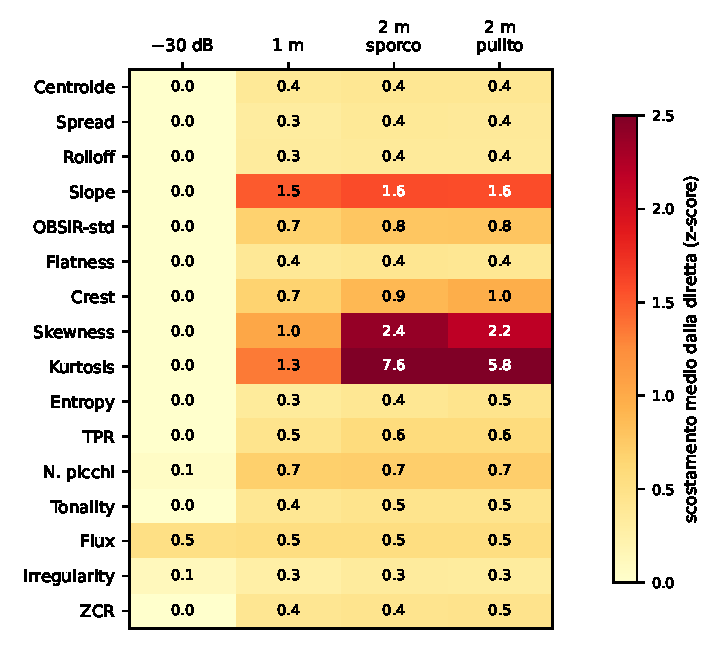
\includegraphics[width=\columnwidth]{figura_scostamento.pdf}}
 \caption{Per ciascun descrittore (righe), lo scostamento medio in z-score fra la
          ripresa diretta e ciascuna configurazione di ripresa (colonne: $-30$~dB di
          controllo, 1~m, 2~m con e senza voci di sottofondo), mediato sui quarantacinque segnali
          sintetici: è la Tabella~\ref{tab:deriva} aperta descrittore per descrittore.
          Chiaro = stabile sotto ripresa, scuro = variabile.}
 \label{fig:scostamento}
\end{figure}

%Il terzo messaggio è quello che più conta portare a casa: una tassonomia di robustezza in tre fasce. Nella fascia alta, stabili in ogni configurazione, stanno flatness, tonality (il suo complemento, quanto lo spettro è tonale), ZCR (il tasso di attraversamenti dello zero, l'unico nel dominio del tempo) e TPR; nella media, che degradano pur mantenendo un'informazione utile, centroide, spread, rolloff, slope, flux e irregularity; nella bassa, instabili a distanza o a basso livello, crest, skewness, kurtosis e numero di picchi.

La terza osservazione riguarda quali descrittori si spostano di più: il crest è per natura un descrittore di contrasto, che misura il rapporto fra picco e pavimento ed è perciò sensibile alla posizione del microfono, mentre skewness e kurtosis sono momenti statistici di ordine elevato, ipersensibili alle code della distribuzione spettrale. La Figura~\ref{fig:scostamento} apre lo scostamento descrittore per descrittore: vi si distingue la quantità dello spostamento dalla sua prevedibilità, perché lo slope, fra i più mossi, si sposta in modo sistematico (negativo, qualunque sia il segnale).
A questo si affianca un sotto-risultato dalla natura paradossale: il caso limite numerico del bin esatto. Su sinusoidi digitali ideali, allineate esattamente a un bin della FFT, alcuni descrittori restituiscono valori anomali (una flatness di 0,945, un TPR di +85 dB, uno spread di 8 Hz, un crest di 1,5). È la formula stessa a degenerare quando le componenti attive sono pochissime: nel limite di una sola bin attiva ($N\to1$) media geometrica e aritmetica coincidono, dunque flatness e crest tendono a $1$, mentre con tutta l'energia in una sola bin lo spread tende a $0$. I valori misurati sono il quasi-limite di questa degenerazione. Gli artefatti scompaiono però non appena interviene una catena acustica, che aggiunge componenti spurie, fa crescere $N$ e rompe la degenerazione: il caso ideale è proprio quello più fragile.

\subsection{Strumenti acustici}\label{sec:strumenti}
Sugli strumenti acustici la domanda cambia: quali descrittori si muovono con la dinamica, e se lo facciano allo stesso modo sui due strumenti.
 Sul clarinetto contrabbasso la dinamica si riflette soprattutto su centroide, rolloff e irregularity (Tabella~\ref{tab:clarinetto}): dal piano al forte crescono in modo monotono, e la flatness li segue con un aumento di circa il sessanta per cento. Tonality e kurtosis si muovono nella direzione opposta; la kurtosis in particolare parte da un valore molto elevato nel piano e crolla nel forte, segno della sua ipersensibilità alle code della distribuzione spettrale. Il crest resta piatto al variare della dinamica: dopo il filtraggio del rumore di fondo il suo andamento non è monotono, conferma concreta della sua bassa robustezza. Anche questi valori sono medie su pochi campioni in una sola sala: vanno presi come indicativi del meccanismo, non come stime di popolazione. La kurtosis 667 del piano, per esempio, è dominata da pochi frame.

\begin{table}[t]
\centering
\small
\begin{tabular*}{\columnwidth}{@{\extracolsep{\fill}}lrrr@{}}
\toprule
 & piano & mezzoforte & forte \\
\midrule
Centroide (Hz) & 218  & 419  & 1162 \\
Rolloff (Hz)   & 309  & 674  & 2137 \\
Irregularity   & 153  & 304  & 977  \\
Flatness       & 0,12 & 0,14 & 0,19 \\
Tonality       & 0,15 & 0,14 & 0,12 \\
Kurtosis       & 667  & 211  & 14,4 \\
\bottomrule
\end{tabular*}
\caption{Clarinetto contrabbasso: i descrittori al variare della dinamica (medie sui frame validi, dopo gate).}
\label{tab:clarinetto}
\end{table}

Sul timpano aumentato, in regime di tono sostenuto, la situazione cambia (Tabella~\ref{tab:timpano}): centroide e rolloff restano fermi mentre la dinamica varia, e la variazione di intensità si legge quasi soltanto dall'irregularity, in modo subordinato dal flux. Sono gli unici due descrittori non invarianti di scala, dunque gli unici capaci di reagire a una variazione di solo livello. Lo spread sembra fare eccezione nel piano, ma è un artefatto della banda piena: la sua media è gonfiata da pochi frame d'attacco, mentre il valore tipico (la mediana, attorno a 17 Hz) resta fermo. Il TPR distingue le dinamiche in modo peculiare: il piano risulta più tonale del forte, perché nel forte l'energia si distribuisce su molte più componenti, riducendo la quota nei picchi tonali. L'entropy resta ferma attorno a 0,11. In un caso limite ancora più severo, un gesto di crescendo e diminuendo applicato al solo livello del tono sostenuto sfugge a tutti i descrittori di forma (centroide, rolloff, crest e tonality restano al valore di base): lo traccia la sola irregularity, che sale e ridiscende con il gesto (da 57 a 79 e ritorno a 46).

\begin{table}[t]
\centering
\small
\begin{tabular*}{\columnwidth}{@{\extracolsep{\fill}}lrrr@{}}
\toprule
 & piano & mezzoforte & forte \\
\midrule
Centroide (Hz)            & 98  & 99  & 109 \\
Spread (Hz)               & 102 & 34  & 52  \\
Rolloff (Hz)              & 106 & 107 & 121 \\
Irregularity              & 39  & 50  & 74  \\
Flux ($\times 10^{-4}$)   & 3,4 & 6,3 & 9,5 \\
Entropy                   & 0,11 & 0,11 & 0,11 \\
\bottomrule
\end{tabular*}
\caption{Timpano aumentato, regime sostenuto: i descrittori al variare della dinamica (medie sui frame validi, dopo gate).}
\label{tab:timpano}
\end{table}

Da questa prova sugli strumenti ricavo che il descrittore che segue il gesto dipende dallo strumento: la forma per il clarinetto, l'irregularity per il timpano sostenuto. È uno dei sostegni della domanda che guida il lavoro: se nessun descrittore è il "giusto" in assoluto, il controllo non potrà sceglierne uno solo a priori, e dovrà tenerli tutti.
Quell'insieme chiuso non è nato però così: lungo il percorso ho scambiato alcune voci, a numero fisso. Ho tolto lo spectral decrease \cite{peeters2004largeset}, ridondante con lo slope, sostituendolo con l'OBSIR-std \cite{essid2006musical} (varianza del decadimento fra ottave, aspetto ortogonale); e ho sostituito il massimo dell'autocorrelazione con l'entropia spettrale di Shannon normalizzata \cite{shen1998robust,misra2004spectral}, che separa meglio i segnali armonici complessi dove flatness e crest saturano. Due ridondanze restano consapevolmente: il tonality coefficient (trasformazione monotona della flatness) e il rolloff (versione robusta del centroide), perché su certi segnali divergono in modo utile. Il criterio è robustezza all'ambiente e ortogonalità, dentro il vincolo dell'insieme chiuso.

\subsection{La terza prova: la distanza}\label{sec:leap}

\begin{figure}[t]
 \centering
 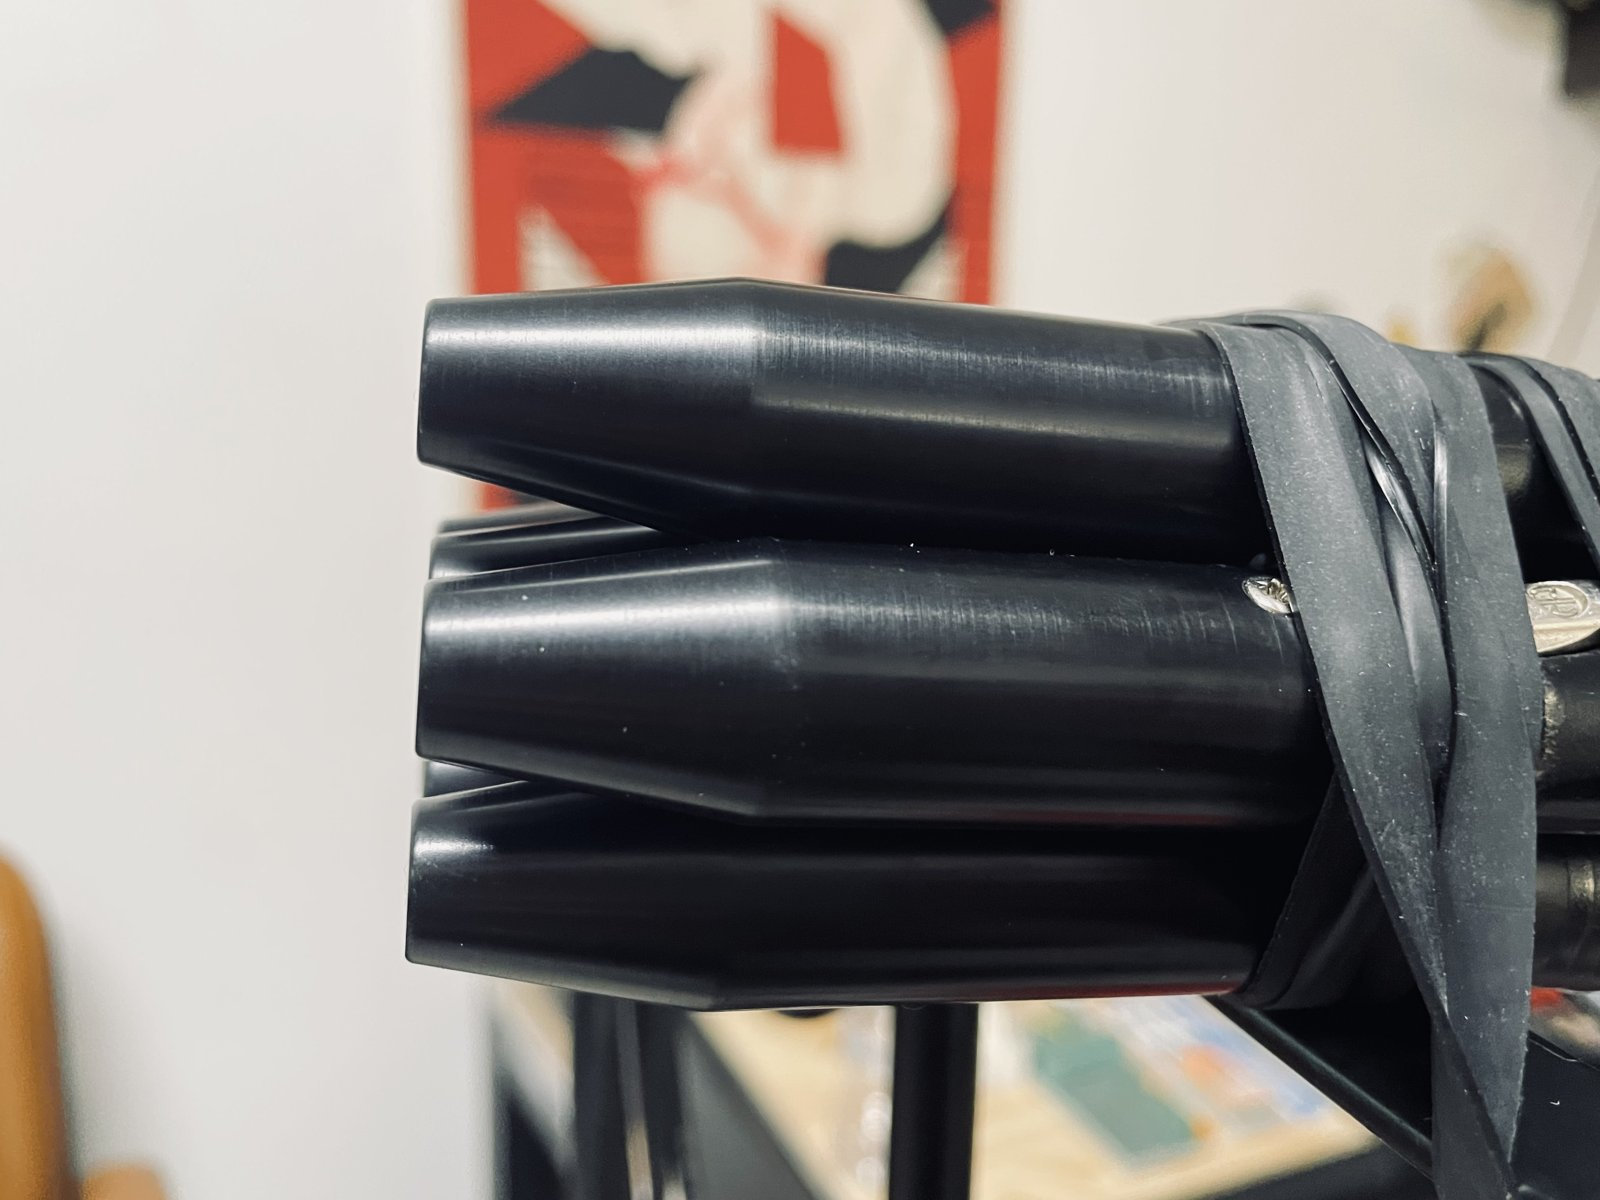
\includegraphics[width=0.48\columnwidth]{foto_apparato.jpg}\hspace{0.6em}%
 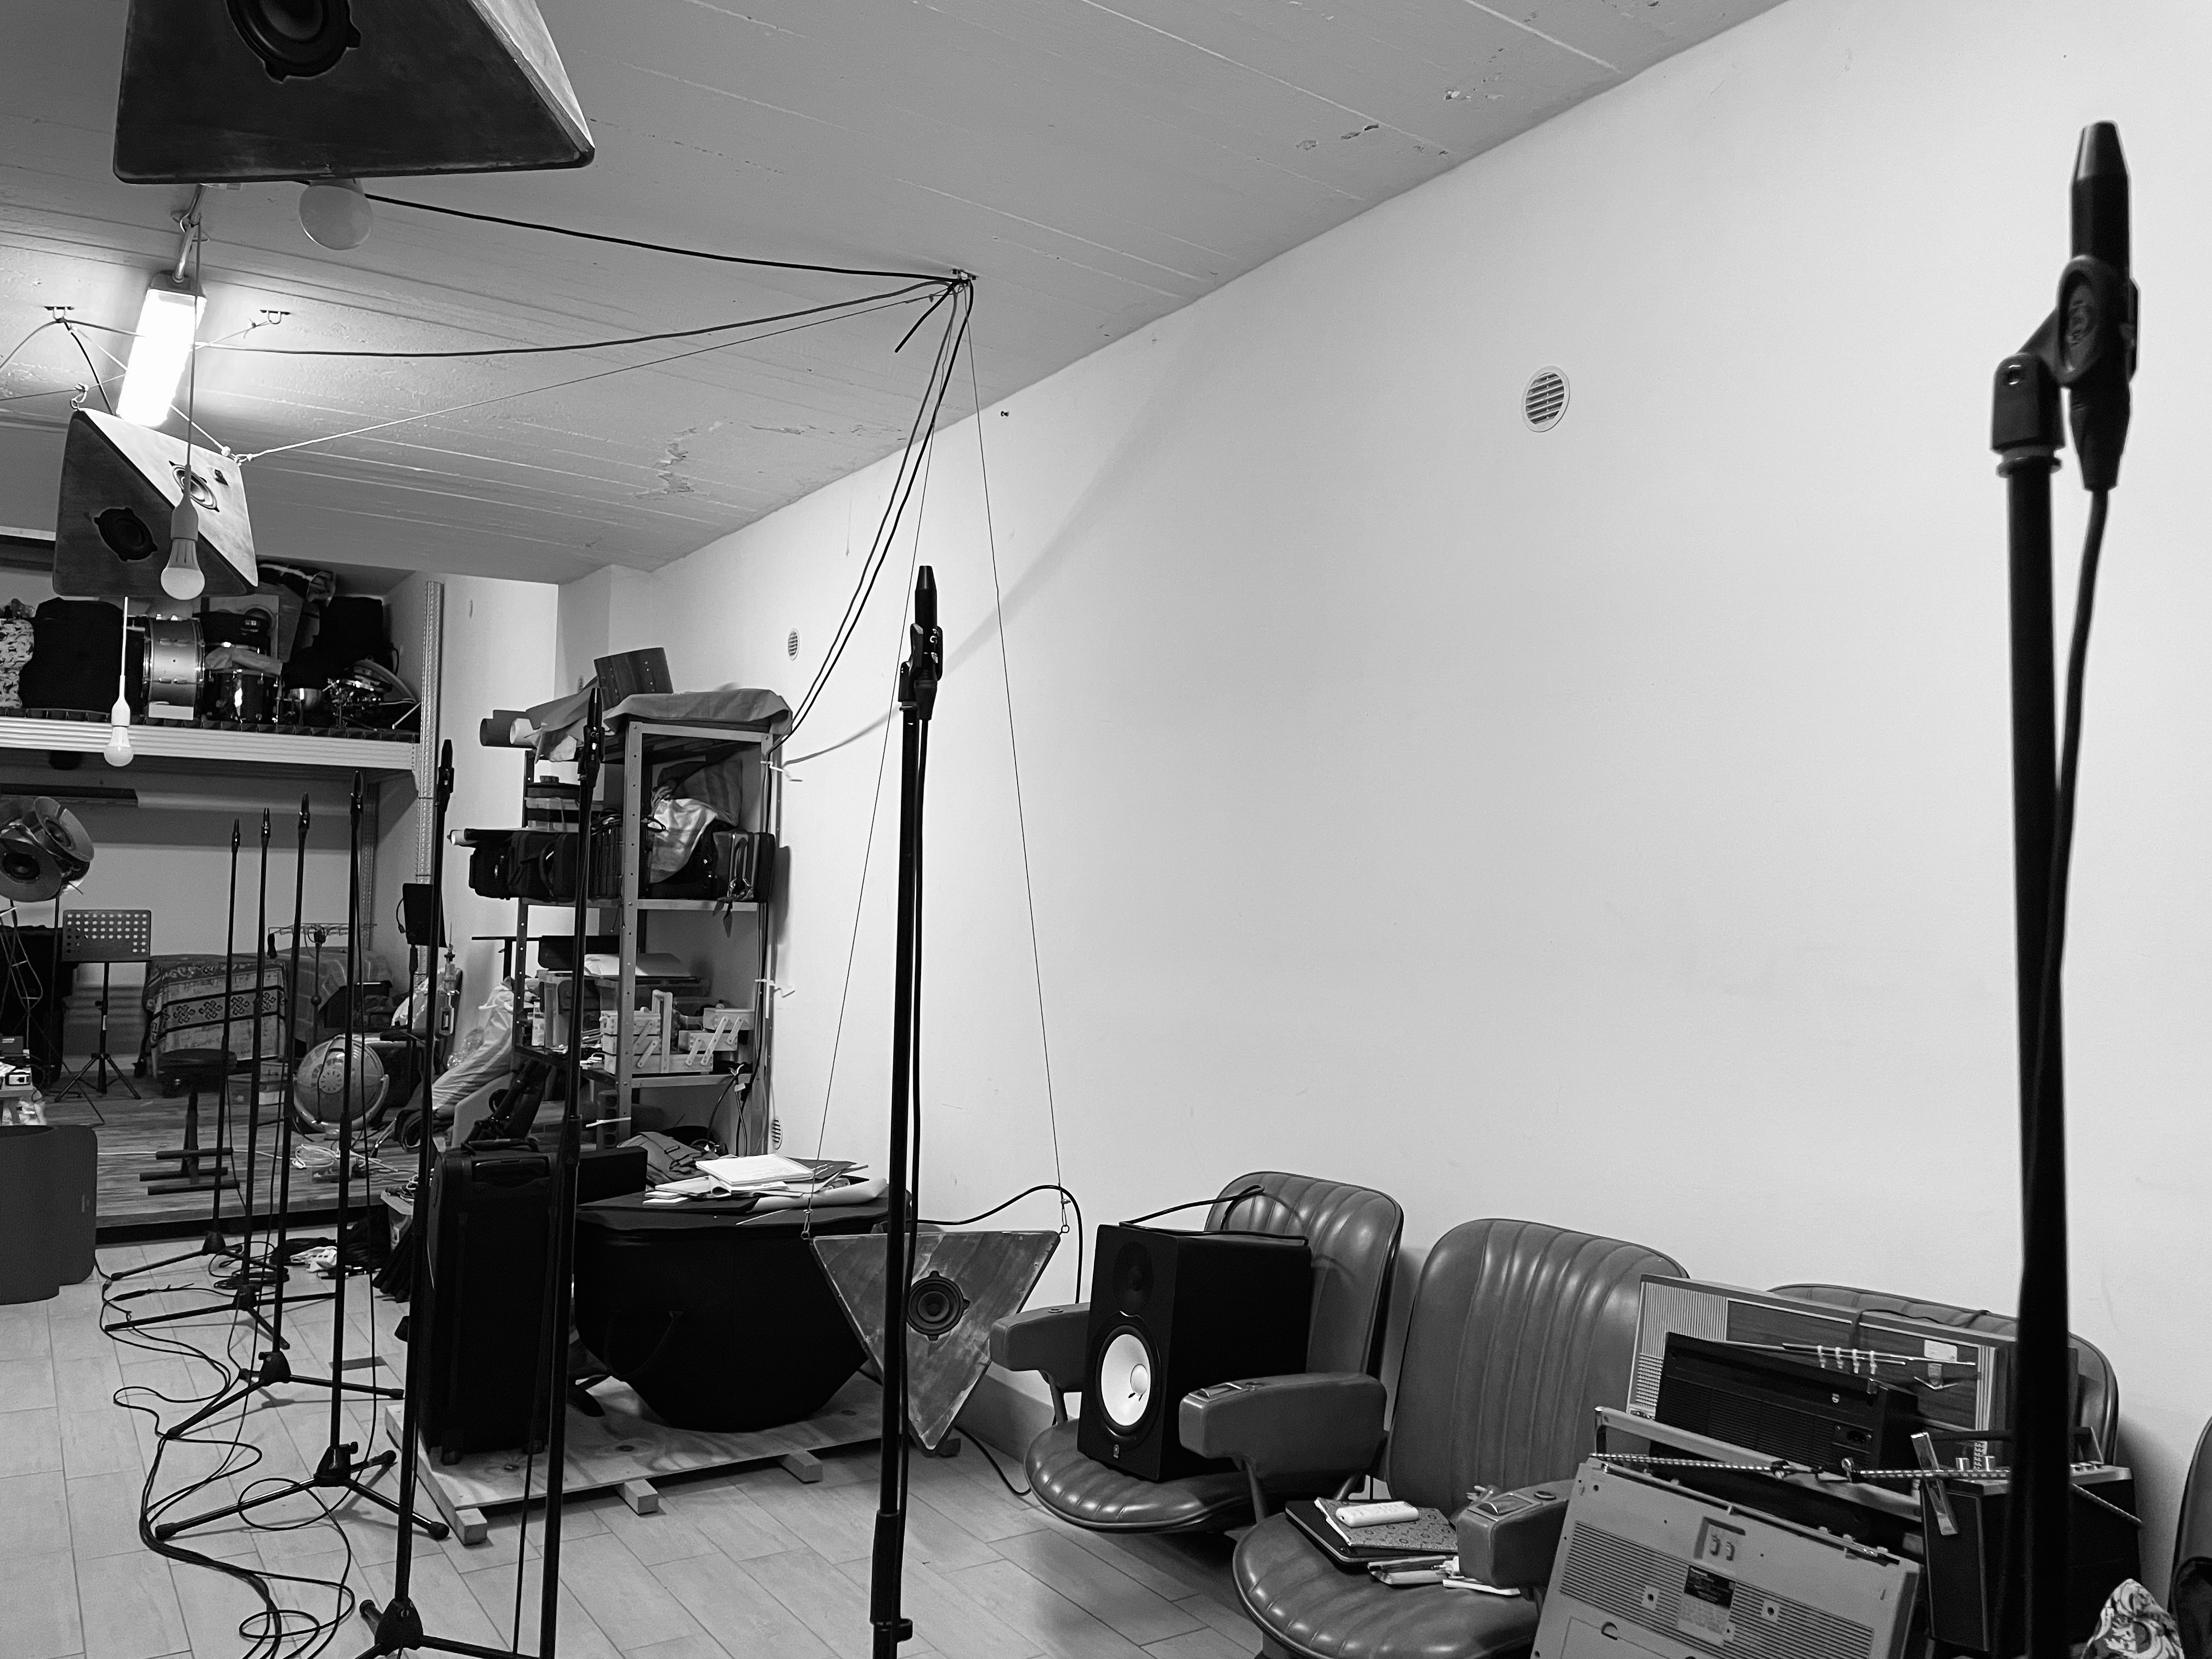
\includegraphics[width=0.48\columnwidth]{foto_fila.jpeg}
 \caption{Apparato della terza prova. A sinistra gli otto microfoni a grappolo, per calibrarne i guadagni a distanza minima fra le capsule; a destra distesi in fila a passi di un metro, da uno a otto metri dalla sorgente.}
 \label{fig:apparato}
\end{figure}

\begin{figure*}[t]
 \centerline{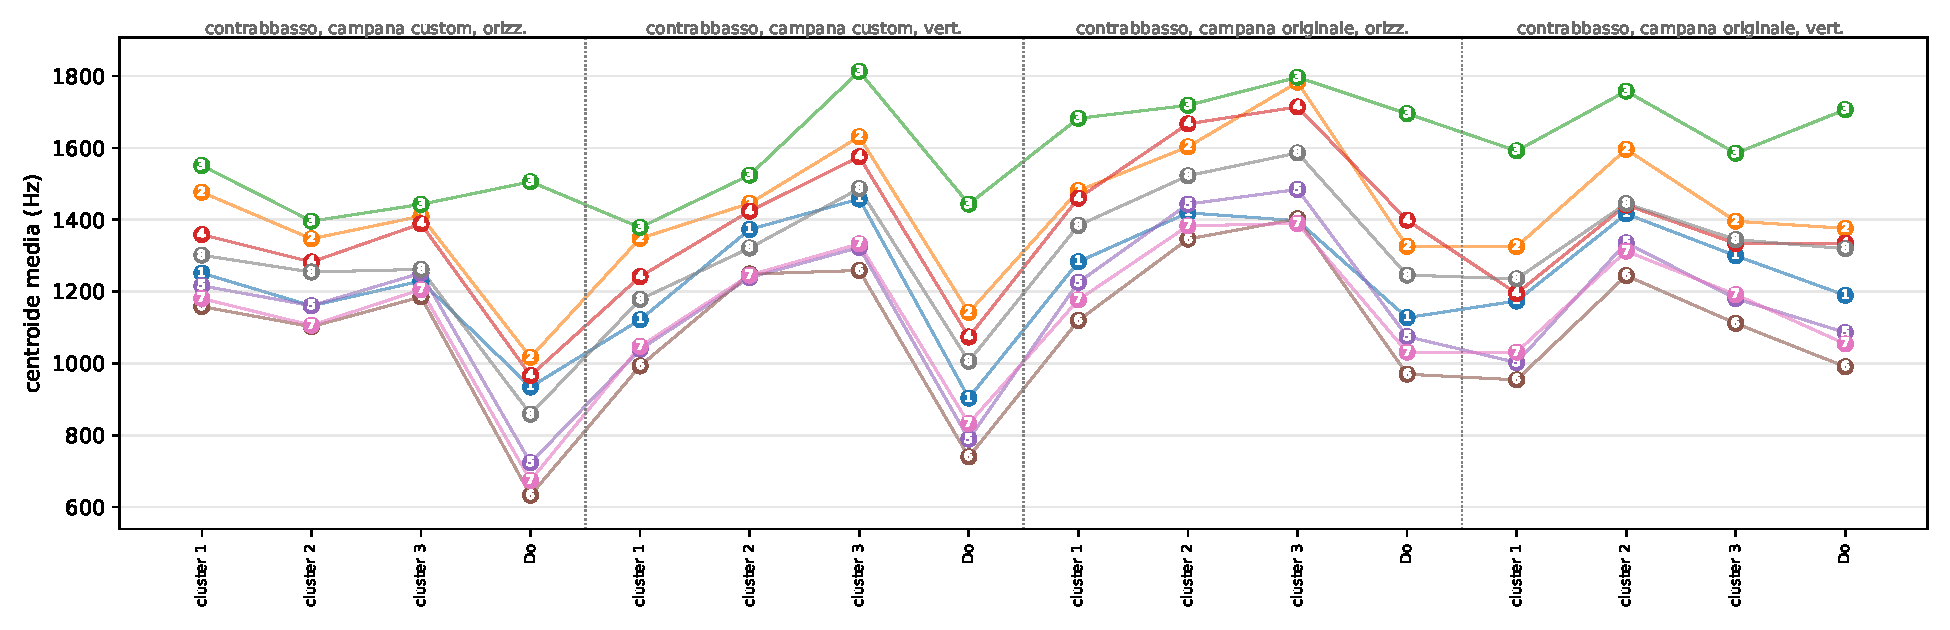
\includegraphics[width=0.85\textwidth]{figura_leap_corpus.pdf}}
 \caption{Il clarinetto contrabbasso nel terzo esperimento: per ogni campione (colonna: le due campane, il trombino originale e il PETALONIO, nei due orientamenti del microfono) il centroide medio a banda piena agli otto microfoni; le linee uniscono lo stesso microfono fra i campioni (numero e colore del punto: vedi legenda).}
 \label{fig:leap_corpus}
\end{figure*}

\begin{figure}[tbp]
 \centerline{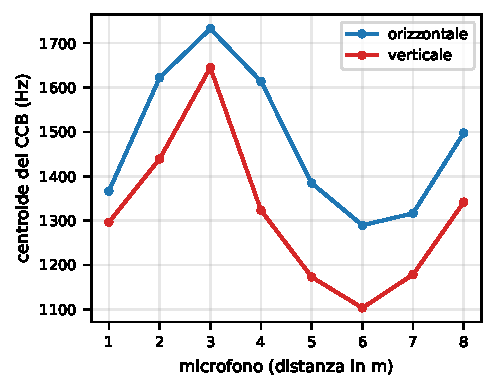
\includegraphics[width=0.74\columnwidth]{figura_leap_onda_ccb.pdf}}
 \caption{Onda stazionaria della fondamentale del clarinetto contrabbasso nella stanza:
          il centroide medio dei cluster lungo gli otto microfoni (a passi di un metro),
          nelle riprese orizzontale (capsula verso la sorgente) e verticale (ortogonale).
          Cresta al microfono~3 (nodo di pressione), avvallamento ai microfoni 5--6 (ventre).}
 \label{fig:leap_onda}
\end{figure}

%La linea di base mi ha portato fin sotto microfono, in sala, ma con una sorgente alla volta e una distanza alla volta.
Per vedere la catena al lavoro in modo sistematico ho preparato la prova centrale, a LEAP, Laboratorio ElettroAcustico Permanente. Ho usato otto microfoni omnidirezionali (Figura~\ref{fig:apparato}), prima raggruppati stretti e poi distesi in fila a passi di un metro, da uno a otto metri dalla sorgente (il canale $n$ corrisponde a $n$ metri), e li ho collegati a un preamplificatore multicanale. Come sorgente ho usato dapprima un altoparlante, con rumore rosa, poi strumenti acustici: un clarinetto contrabbasso (un Do grave a tubo chiuso e un cluster) e un clarinetto soprano (un cluster). Il clarinetto contrabbasso l'ho registrato sia con la sua campana originale rivolta in avanti sia con il PETALONIO\footnote{Campana alternativa a quella svasata originale, costruita da Giuseppe Silvi, più scura e più appuntita: il centroide del Do sta a 952 Hz contro 1250.}, un trombino verticale rivolto verso l'alto. Ogni campione l'ho registrato due volte, con i microfoni in orizzontale (le capsule rivolte verso la sorgente) e in verticale (puntati verso l'alto), per separare la propagazione dell'onda dalla direttività propria del microfono. I guadagni li ho calibrati perché gli otto canali restituissero lo stesso RMS sul cluster di calibrazione. %l'allineamento è risultato ottimo, con una deviazione standard di 0,17 dB sugli otto canali.


La Figura~\ref{fig:leap_corpus} dà il quadro d'insieme dei campioni di clarinetto contrabbasso: il centroide si sposta vistosamente da un punto di ripresa all'altro.

%Il filo conduttore è il centroide. Per costruzione è invariante al guadagno, come ho dimostrato nella linea di base (Sezione~\ref{sec:basale}): scalando lo spettro per un fattore qualsiasi, il suo valore non cambia.
Il centroide è invariante al guadagno, e ne segue un fatto prezioso: se cambia passando da un microfono all'altro, quel cambiamento non è livello, è lo spettro che la catena deforma lungo il tragitto.

La prima osservazione riguarda la perdita di acuti con la distanza. A banda intera il centroide del rumore scende nettamente con la distanza: in orizzontale da circa 8970 Hz a un metro fino a circa 5700 Hz a otto metri, all'incirca un terzo in meno; in verticale da circa 6300 a circa 5000 Hz. Ma limitando l'analisi a 10 kHz lo stesso centroide appare quasi piatto, attorno a 3500 Hz e appena mosso, perché la perdita è tutta negli acuti oltre i 10 kHz: l'aria assorbe le frequenze alte lungo il tragitto, e un tetto a 10 kHz lo nasconderebbe. Nella stessa direzione spingono però anche la direttività della sorgente e il campo riverberato, che questi dati confondono con l'assorbimento.

La seconda osservazione è un'onda stazionaria sul clarinetto contrabbasso (Figura~\ref{fig:leap_onda}). Sui suoi cluster il centroide, mediato sui campioni, disegna un'onda lungo gli otto microfoni: una cresta attorno al microfono 3, un avvallamento attorno ai microfoni 5 e 6. Le curve orizzontale e verticale quasi coincidono nella forma, e questo esclude che sia direttività del microfono: è un'onda stazionaria della fondamentale del clarinetto nella stanza. Vicino al microfono 3 c'è un nodo di pressione, dove la fondamentale è debole e il centroide perciò sale; vicino ai microfoni 5 e 6 c'è un ventre, dove la fondamentale è forte e il centroide perciò scende. La geometria torna: il quarto d'onda di circa due metri e mezzo fra nodo e ventre dà una frequenza attorno ai 34 Hz, dentro il registro grave dello strumento. Il clarinetto soprano non mostra quest'onda, perché la sua fondamentale più acuta ha nodi e ventri a passo più fitto.

\begin{figure*}[t]
 \centerline{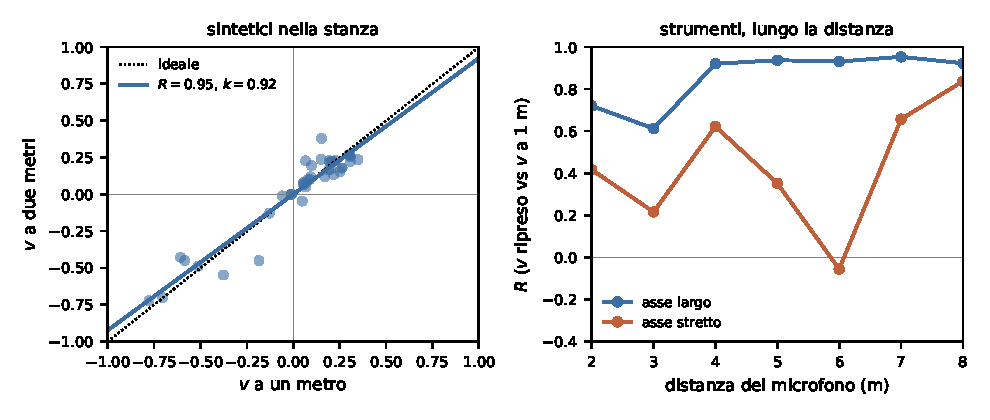
\includegraphics[width=0.82\textwidth]{figura_controllo_nodi.pdf}}
 \caption{Il controllo a nodi nella stanza, in z-score. A sinistra, sui sintetici:
          $v$ a due metri contro $v$ a un metro (entrambi ripresi, nodi a un metro).
          A destra, sugli strumenti lungo la distanza: $R$ fra $v$ ripreso e $v$ a un metro,
          su un asse largo fra registri (blu) e uno stretto fra suoni dello stesso strumento (rosso).}
 \label{fig:controllonodi}
\end{figure*}



%La terza osservazione riguarda l'attenuazione. L'RMS del rumore scende con la distanza in modo dolce: ho misurato circa $-8{,}6$ dB a otto metri in orizzontale, cioè circa $-2{,}9$ dB per raddoppio, confermato da un fonometro nella stanza (96/93/90/87 dBA a 1/2/4/8 metri, esattamente $-3$ dB per raddoppio). L'ampiezza segue dunque la legge $1/\sqrt{r}$: il contributo riverberante della sala, che decade poco con la distanza, si somma al suono diretto e ne ammorbidisce la caduta.

\medskip\noindent\textbf{La risposta degli altri descrittori.}\quad
L'oscillazione non riguarda però il solo centroide. Sugli stessi cluster ho correlato il profilo per canale di ciascun descrittore con quello del centroide, per misurare quanti condividano l'oscillazione fra nodo di pressione e ventre (Tabella~\ref{tab:onda}). La portano in dodici sui sedici: il centroide stesso, che è la sonda, più undici altri. Sette si muovono in fase con esso, più acuti dove la fondamentale è debole, con correlazioni fra 0,92 e 0,98; quattro si muovono in opposizione, da $-0{,}82$ a $-0{,}96$, perché dove la fondamentale è debole leggono meno dominanza tonale e meno picco; gli altri quattro restano indifferenti. La lettura è semplice: nodo e ventre sono un'unica leva, la forza della fondamentale, e tutto ciò che pesa l'equilibrio fra fondamentale e resto si muove con essa. Quali descrittori portino l'onda non è deducibile da cosa ciascuno misura: il centroide la porta ma l'OBSIR-std no, ZCR e irregularity la portano ma il flux no, e descrittori per altri versi vicini finiscono su lati opposti. La domanda utile è una sola, se un descrittore risponda o meno alla fondamentale.

\begin{table}[tbp]
\centering
\small
\begin{tabular*}{\columnwidth}{@{\extracolsep{\fill}}lp{3.4cm}@{}}
\toprule
Rispetto all'onda & Descrittori (corr. col centroide) \\
\midrule
In fase & zcr, rolloff, skewness, entropy, spread, irregularity, tonality (0,92 … 0,98) \\
\addlinespace
In opposizione & tpr, flatness, slope, crest ($-0{,}82$ … $-0{,}96$) \\
\addlinespace
Indifferenti & kurtosis, flux, OBSIR-std, n. picchi ($|r|<0{,}5$) \\
\bottomrule
\end{tabular*}
\caption{Quali descrittori portano l'onda di pressione sul clarinetto contrabbasso: correlazione del profilo per canale col centroide, su $n=8$ microfoni.}
\label{tab:onda}
\end{table}

Un secondo segno lo lascia la campana sul Do tenuto. La kurtosis, indifferente all'onda sui cluster, sul Do sale da circa 21 al nodo di pressione a quasi 60 al ventre quando il PETALONIO è puntato di fronte alla capsula, mentre con la campana originale, o con la stessa campana e capsula ruotata, resta fra 10 e 13. Occorre il concorso di tre condizioni (la nota singola, il ventre dove la fondamentale è forte, il PETALONIO): la kurtosis indica qui l'interazione fra campana, luogo e microfono, più che la distanza.

\medskip\noindent\textbf{Direttività e sorgente.}\quad
Resta la direttività del microfono, e la doppia ripresa la isola. Ruotando la capsula da orizzontale a verticale, sul clarinetto contrabbasso quasi nessun descrittore cambia oltre l'otto per cento (centroide, spread e rolloff entro il quattro): lo strumento ha poca energia negli acuti, dove la direttività del microfono agisce. La si vede invece sul rumore a banda larga, dove il centroide orizzontale parte molto più alto del verticale, perché la capsula rivolta verso la sorgente raccoglie più acuti. Il clarinetto soprano ha il profilo per canale piatto, entro circa $\pm 80$ Hz attorno a una media di circa 1740 Hz, più alta del contrabbasso (fra 1180 e 1600 Hz). Che l'onda compaia sul contrabbasso e non sul soprano dice che la sorgente entra nel conto accanto al luogo.

\medskip\noindent\textbf{Nota matematica.}\quad
Una relazione regge le altre letture: l'attenuazione in sala è di $-3$ dB a ogni raddoppio della distanza, perché il riverbero ammorbidisce la caduta rispetto al campo libero ($20\log_{10}(1/\sqrt{2})\approx-3$ dB, confermato dal fonometro).

La catena è coautrice della misura: l'ambiente, la distanza e il microfono entrano nel numero. È la conclusione comune alle tre prove, e da qui nasce la domanda pratica: se il valore assoluto di un descrittore porta dentro di sé la catena, come lo si usa dal vivo? La via che propongo è nella sezione~\ref{sec:nodi}. %Resta un dubbio aperto: se l'onda stazionaria sia un modo fisso della stanza o dipenda dalla posizione della sorgente; una prova futura sposterebbe la sorgente per vedere se il nodo cade nello stesso punto.


\section{Una proposta esplorativa: dal descrittore al controllo a nodi}\label{sec:nodi}

Serve dunque una misura relativa, perché il valore assoluto porta dentro di sé la catena. È il limite dei cinque descrittori iniziali di \brano: ogni parametro era guidato dal valore assoluto di un descrittore, e quel valore si spostava con l'ambiente invece che col gesto.
 La via d'uscita sta nel cambiare ciò che si legge: la posizione del segnale rispetto a due suoni di riferimento, i nodi, al posto del valore di un singolo descrittore. Al posto di un descrittore per parametro, un asse a nodi per parametro.

Il controllo che ne risulta è bipolare: il valore di controllo $v$ nasce dal rapporto fra le distanze del punto dai due nodi, secondo l'Equazione~\eqref{eq:ancore}, dove $d_{+}$ e $d_{-}$ sono rispettivamente la distanza dal polo $+1$ e dal polo $-1$.

\begin{equation}
  v \;=\; \frac{d_{-} - d_{+}}{d_{-} + d_{+}} \;\in\; [-1,\,1]
  \label{eq:ancore}
\end{equation}

Il valore con segno $v$ vale $+1$ sul prototipo positivo, $-1$ su quello negativo, $0$ a metà strada. Ogni nodo è il vettore dei sedici descrittori del suono di riferimento, mediati sui suoi frame; le distanze sono euclidee in quello spazio, normalizzato a z-score congelato (Sezione~\ref{sec:basale}), con tutti i descrittori a peso uguale.


%\begin{figure}[tbp]
 %\centerline{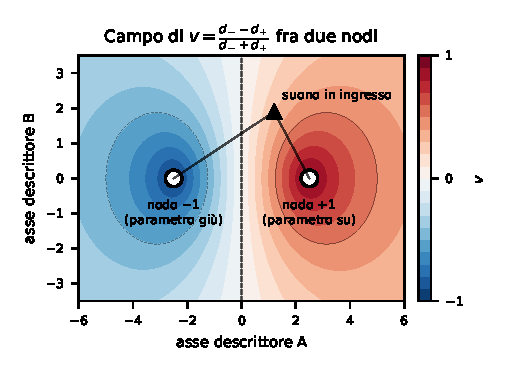
\includegraphics[width=\columnwidth]{figura_ancore.pdf}}
 %caption{Il controllo a nodi: il valore con segno $v$ nasce dal rapporto fra le
%        distanze del punto dai due poli ($+1$ e $-1$) nello spazio dei
%          descrittori, e vale $0$ a metà strada.}
%\label{fig:ancore}
%\end{figure}

%Un punto va dichiarato con chiarezza:
Sono i nodi a definire l'asse, e il controllo legge soltanto la posizione del punto lungo quell'asse, restando cieco a ciò che gli è ortogonale. La scelta dei nodi è perciò una decisione compositiva. Se si fissano due suoni dello stesso strumento, per esempio un piano e un forte di clarinetto, l'asse è quella dinamica, e un punto che si muove in tutt'altra direzione vi resta vicino allo zero: la sua variazione cade fuori dall'asse scelto. Due sorgenti diverse, invece, misurano quanto un segnale pende verso l'una o verso l'altra. Una condizione necessaria è la raggiungibilità: l'asse deve essere percorribile dal segnale in ingresso, altrimenti il controllo non produce variazione. %Tutto questo è coerente con la tesi di un insieme chiuso di sedici descrittori: i descrittori restano sempre gli stessi, a cambiare sono soltanto i due prototipi e la scala con cui si misurano le distanze.

Il meccanismo del metodo è che il contesto entra alla pari in entrambi i termini del confronto. Se prendo i due nodi nello stesso ambiente e con la stessa catena del segnale in ingresso, la firma del luogo che la prova della distanza ha reso visibile (l'aria che toglie gli acuti, l'onda stazionaria della fondamentale) grava in egual misura sul segnale e sui suoi riferimenti, e nel rapporto fra le distanze si bilancia: la catena, coautrice del numero, diventa il fondo comune su cui si legge il gesto invece di confondersi con esso.

%Ho voluto mettere questa relatività alla prova invece di darla per buona.
 Per ciascuno dei quarantacinque sintetici ho confrontato il valore di $v$ a un metro con quello a due metri, entrambi ripresi nella stanza, con i due nodi tarati una volta nell'ambiente a un metro. È la condizione del vivo: l'ingresso e i nodi vivono nello stesso ambiente, non esiste un riferimento asciutto. I punti restano sulla diagonale (Figura~\ref{fig:controllonodi}, a sinistra), con correlazione intorno a $0{,}95$ e pendenza vicina a $0{,}9$: la lettura a due metri quasi coincide con quella a un metro. Misurati sullo stesso passaggio e con la stessa statistica, i descrittori assoluti si spostano poco, mentre kurtosis e skewness derivano nettamente (bias di $+3{,}3$ e $+1{,}0$ in z-score). Sui sintetici $v$ resta centrato, e prescinde dal sapere in anticipo quali descrittori quel luogo lascerà fermi; sugli strumenti lungo la distanza conserva l'ordine dei segnali ma non il proprio livello. La coppia sinusoide/rumore percorre però l'asse di massima varianza, il più facile da conservare. Fra i sintetici una coppia di modulazioni di frequenza si conserva (R attorno a 0,6--0,7), una di miscele tonale/rumore si appiattisce e a due metri si inverte.

Sugli strumenti, lungo le otto distanze (Figura~\ref{fig:controllonodi}, a destra), su un asse largo, fra due clarinetti di taglia diversa (contrabbasso grave e soprano) la correlazione fra la lettura ripresa e quella a un metro resta intorno a 0,9 fino a otto metri, mentre su un asse stretto fra suoni dello stesso strumento la lettura si fa irregolare: tiene fra 0,4 e 0,8 quasi ovunque e tocca lo zero solo al microfono 6, il ventre dell'onda stazionaria.

Questi numeri indicano il meccanismo più che la portata del controllo: li ho misurati su segnali registrati per studiare la catena, non per saggiare i nodi. Un cluster, poi, non è un punto fermo: al suo interno il suono si muove di continuo, e trattarlo come riferimento unico è una semplificazione.

Il crollo al microfono 6 mostra la condizione di validità del metodo. Il bilanciamento richiede che la firma del luogo gravi in egual misura sul segnale e sui due nodi. Al ventre dell'onda la fondamentale è forte, e la Tabella~\ref{tab:onda} mostra che dodici descrittori su sedici rispondono proprio alla sua forza. Su un asse largo, fra registri diversi, i due nodi stanno da parti opposte rispetto a quella leva e lo spostamento resta comune ai due termini del rapporto. Su un asse stretto, fra suoni dello stesso strumento, i due nodi condividono la fondamentale: l'onda li muove quasi insieme, la differenza fra le due distanze si assottiglia, e con essa l'informazione che $v$ trasporta. Al ventre $v$ non sbaglia il numero: lì il segnale è davvero un altro. A venire meno è la coincidenza fra ciò su cui poggia l'asse e ciò su cui agisce il luogo, che conta più della distanza fra i nodi: su un asse stretto è il luogo stesso a occupare l'asse. Scegliere un asse è perciò anche scegliere a quale leva della stanza si resta esposti, e dove cade il microfono è parte della taratura (Sezione~\ref{sec:discussione}).

Da questa condizione ricavo due criteri. Il primo è dove cadono i nodi rispetto ai segnali in ingresso. Con una sinusoide e un rumore bianco come poli, i gesti di clarinetto e timpano restano fra $+0{,}1$ e $+0{,}3$, lontani da entrambi i lati: l'asse è definito, ma il segnale ne percorre una frazione. Riprendere i due poli con la stessa catena dell'ingresso, che è già la regola per entrambi i nodi, non cambia questo: la loro collocazione dipende da quali suoni sono, non da come sono stati registrati. Nodi presi fra i suoni dello stesso mondo dell'ingresso lasciano invece al segnale l'intervallo fra $-1$ e $+1$, ed è con questi che vale la tenuta della Figura~\ref{fig:controllonodi}.

Il secondo è la metrica, perché la tenuta vale per la distanza euclidea sugli z-score e non per lo sbiancamento di Mahalanobis~\cite{mahalanobis1936generalised}: è piuttosto uno strumento diagnostico da usare in fase di taratura, non una correzione da applicare sempre. Amplificando flux e irregularity, i descrittori di varianza ridotta nel corpus, lo sbiancamento dà peso proprio all'irregolarità che l'ambiente aggiunge, e sotto ripresa il controllo si conserva meno.

Il metodo ha poi un costo, e va dichiarato: i sedici descrittori si riducono a una sola distanza, e il valore di $v$ tace quale proprietà dello spettro si sia mossa. È voluto: sapere quale descrittore ha reagito serve quando si scelgono i nodi e si verifica su cosa poggia l'asse, mentre dal vivo serve un valore solo lungo l'asse scelto. E i sedici entrano tutti nella distanza, compresi i più fragili sotto catena (crest, skewness, kurtosis, numero di picchi), perché quali descrittori portino un dato asse si sa solo a posteriori (lo mostra l'onda di pressione). Una pesatura per-asse è il raffinamento naturale.

Su questa base l'idea si estende a più dimensioni: più coppie di nodi, ciascuna col proprio asse, generano più valori $v$ simultanei dallo stesso ingresso, cioè una superficie di controllo i cui assi sono direzioni musicali scelte in calibrazione o ridefinite lungo il brano. È il controllo con cui in \brano guido il comportamento elettronico dal vivo. Nell'anello ecosistemico il sistema legge la propria posizione rispetto a riferimenti che vivono nello stesso ambiente e si muovono con esso.

I nodi, inoltre, possono cambiare dal vivo: il sistema può promuovere a nodo il segnale ripreso in un istante, la media degli ultimi secondi suonati, o un suono sintetico verso cui tendere. Cambiare un nodo ribalta tutti i rapporti, perché il segnale si misura di colpo rispetto a un altro riferimento: un'articolazione strutturale del brano.

Anche la distanza fra i nodi resta infine una scelta di progetto: allontanarli rende la lettura robusta ma grossolana, avvicinarli fine ma fragile, fino a due nodi coincidenti dove l'asse si annulla; un criterio sistematico per tararla resta fra i lavori futuri.

\section{Discussione}\label{sec:discussione}

Dal percorso traggo alcuni criteri pratici per chi voglia usare descrittori audio come controllo dal vivo, fuori dal dominio della Music Information Retrieval (MIR) per cui erano stati pensati. Il primo è un cambio di sguardo: l'ambiente entra nel segnale e lo trasforma, e i descrittori vanno letti lì, dove la robustezza dice quanto una misura si sposta sotto ripresa (uno spostamento ampio ma sistematico resta leggibile). Il criterio è conoscere come ciascun descrittore si comporta nel proprio contesto e valutare, dove serve stabilità al cambio di sala, il passaggio da valori assoluti a misure relative.

Per chi progetta nuove mappature, l'indicazione centrale è che il valore di un descrittore è una grandezza contestuale: dipende dall'ambiente di ripresa e dalla sorgente. La calibrazione è perciò parte integrante del metodo, tanto quanto la scelta dei descrittori, e ha due tempi distinti. Lo z-score si congela una volta sola, sul corpus dei segnali sintetici: normalizza le unità dei descrittori, che non cambiano da una sala all'altra, e si può perciò precaricare. I nodi, invece, sono ciò che si tara in sala, ed è qui che si chiude il ponte verso il tempo reale: dal vivo non esiste un corpus, e la taratura è una breve presa di riferimento prima di cominciare, con la stessa catena microfonica del segnale da misurare, che fissa i due prototipi nell'ambiente reale.

Vanno dichiarati anche i limiti. Il primo è strutturale: nel caso del timpano in regime sostenuto, una variazione di puro livello sfugge ai descrittori invarianti di scala, e fra i due sensibili al livello la registra la sola irregularity, che però il livello se lo porta dentro invece di misurarlo; per leggere la dinamica serve una misura d'intensità accanto ai sedici. Il corpus stesso è ristretto: due strumenti in una sola sala, più un terzo nella terza prova. Le regolarità che riporto descrivono questi casi e il meccanismo che li produce, non altri strumenti o altri luoghi. Il secondo riguarda la portata della validazione del controllo a nodi (Sezione~\ref{sec:nodi}): l'ho saggiata su un corpus raccolto per altri scopi, su pochi campioni e mai dentro il brano con un criterio d'ascolto; resta una prova di principio. Manca un esperimento dedicato, con un cluster fissato come nodo e misurato in tempo reale mentre il clarinetto va da una nota singola verso il cluster, accanto a una ri-normalizzazione del guadagno sotto ripresa. Resta poi il punto aperto sollevato dalla prova della distanza (Sezione~\ref{sec:leap}): se l'onda stazionaria osservata sul clarinetto sia un modo fisso della stanza o dipenda dalla posizione della sorgente; la prova decisiva è spostare la sorgente e vedere se il minimo dell'onda ricade nello stesso punto.

C'è infine un rovesciamento che porto nel brano. L'onda stazionaria che lungo la distanza disturba il controllo è anche una risorsa: gli strumenti dispongono nodi e ventri di pressione nella stanza, e collocare il microfono in un punto scelto decide quali descrittori risponderanno e quali resteranno fermi. La posizione del microfono diventa così una scelta compositiva dentro l'anello ecosistemico, al pari della taratura dei nodi: dove l'ascolto del luogo è il principio dell'ecosistemico, qui il luogo entra nel brano attraverso due decisioni: dove cade il microfono, e fra quali suoni si tendono gli assi.
\bibliography{riferimenti}

\end{document}
